% !TeX program = pdflatex
% !TeX spellcheck = es_ES
% !TeX encoding = utf8
%\documentclass{article}
\documentclass[11pt, a4paper, twoside, openright, openany]{book}
% Math text
\usepackage[utf8]{inputenc}
\usepackage[a4paper,
            top=2cm,bottom=2cm,
            margin=3.5cm,
            headheight=27pt]{geometry}
\usepackage[spanish, mexico]{babel}
%\usepackage[utopia]{mathdesign}
\usepackage{amsmath,amssymb,array,siunitx}
% HEADER
\usepackage{fancyhdr,framed}
\setlength{\headheight}{44pt}
\pagestyle{fancy}
\usepackage[T1]{fontenc}
\usepackage[utf8]{inputenc}
\usepackage{soulutf8,xcolor}
\usepackage{svg}
\usepackage{graphicx}

%\input{tex/testpreamble.tex}
% !TeX root = control_rapido.tex
%% DIFFERENTIAL OPERATOR
\makeatletter
\providecommand*{\diff}%
{\@ifnextchar^{\DIfF}{\DIfF^{}}}
\def\DIfF^#1{%
	\mathop{\mathrm{\mathstrut d}}%
	\nolimits^{#1}\gobblespace}
\def\gobblespace{%
	\futurelet\diffarg\opspace}
\def\opspace{%
	\let\DiffSpace\!%
	\ifx\diffarg(%
	\let\DiffSpace\relax
	\else
	\ifx\diffarg[%
	\let\DiffSpace\relax
	\else
	\ifx\diffarg\{%
	\let\DiffSpace\relax
	\fi\fi\fi\DiffSpace}


\newcommand{\dimfont}[1]{\ensuremath{#1}}
\newcommand{\Cme}[1]{\mathbf{#1}}
\newcommand{\Mme}[1]{\mathbf{#1}}
\newcommand{\Ts}{T_s}

\newcommand{\eye}{\Mme{I}}
%transpose
\def\dt{\Delta t}
\def\tp{^{\top}}
% Small
\def\MA{\Mme{A}}
\def\MB{\Mme{B}}
\def\MC{\Mme{C}}
\def\MD{\Mme{D}}
\def\ME{\Mme{E}}
\def\MK{\Mme{K}}
\def\MW{\Mme{W}}
\def\MX{\Mme{X}}
\def\MV{\Mme{V}}
\def\ctrb{\Mme{Y}}
\def\Mzero{\Mme{0}}
\def\obsv{\Mme{\mathcal{O}}}

\newcommand{\ts}[2]{\left. #1\right|_{\tiny #2}}

\def\error{\varepsilon}
\def\Cx{\Cme{x}}
\def\Cf{\Cme{f}}
\def\Cy{\Cme{y}}
\def\Cu{\Cme{u}}
\def\Cn{\Cme{n}}
\def\Cd{\Cme{d}}
\def\Czero{\Cme{0}}
\def\Cv{\Cme{v}}
\def\Cz{\Cme{z}}
\def\Cw{\Cme{w}}
\def\Jcost{\Cme{\mathcal{J}}}
% RK4
\def\Ca{\Cme{a}}
\def\Cb{\Cme{b}}
\def\Cc{\Cme{c}}


\def\noise{{n}}
\def\disturb{{d}}
\newcommand{\di}{\ensuremath{\textrm{d}}}

\newcommand{\Matlab}{{\sc Matlab}}

\newcommand{\spartial}[2]{\frac{\partial {#1}}{\partial {#2}}}
\newcommand{\dpartial}[2]{\frac{\partial^2 #1}{\partial #2 ^2}}

\usepackage{amsthm}
\theoremstyle{definition}
\newtheorem{definition}{Definition}[chapter]
\newtheorem{theorem}{Teorema}[chapter]
\newtheorem{exercise}{Ejercicio}[chapter]
%\usepackage{bigfoot} % to allow verbatim in footnote
\usepackage[numbered,framed]{matlab-prettifier}

\let\ph\mlplaceholder % shorter macro
\lstMakeShortInline"
\renewcommand{\lstlistingname}{Código}
\renewcommand{\lstlistlistingname }{Códigos \Matlab}
\lstset{
  style              = Matlab-editor,
  basicstyle         = \mlttfamily,
  escapechar         = ",
  mlshowsectionrules = true,
  numbers = none,
  tabsize=4,
  literate = {-}{-}1,
}

  % !TEX encoding = UTF-8 Unicode
  % !TEX root = ../control_rapido.tex
  % !TeX spellcheck = en_EN

\usetikzlibrary{arrows,babel,fit,patterns,decorations.pathmorphing,decorations.markings,calc}
\tikzstyle{block} = [draw, fill=blue!20, rectangle, 
minimum height=3em, minimum width=6em]
\tikzstyle{sum} = [draw, fill=blue!20, circle, node distance=1cm]
\tikzstyle{input} = [coordinate]
\tikzstyle{output} = [coordinate]
\tikzstyle{pinstyle} = [pin edge={to-,thin,black}]
\tikzstyle{ground}=[fill,pattern=north east lines,draw=none,minimum width=0.75cm,minimum height=0.3cm]
\tikzstyle{damper}=[thick,decoration={markings,  
	mark connection node=dmp,
	mark=at position 0.5 with 
	{
		\node (dmp) [thick,inner sep=0pt,transform shape,rotate=-90,minimum width=15pt,minimum height=3pt,draw=none] {};
		\draw [thick] ($(dmp.north east)+(2pt,0)$) -- (dmp.south east) -- (dmp.south west) -- ($(dmp.north west)+(2pt,0)$);
		\draw [thick] ($(dmp.north)+(0,-5pt)$) -- ($(dmp.north)+(0,5pt)$);
	}
}, decorate]
\tikzstyle{spring}=[thick,decorate,decoration={zigzag,pre length=0.3cm,post length=0.3cm,segment length=6}]

% PGF PLOT!

\pgfplotsset{
	table/search path={plots},
}

%    \pgfplotsset{
%        % use this `compat' level or higher to use the LUA backend for calculation
%        % (--> speed improvement)
%        compat=1.12,
%        % declare your function here ...
%        /pgf/declare function={
%%            f(\x,\a) = ((\x)^0.65 + sin(1.5*pi*(\x))) - ((\a)^0.65 + sin(1.5*pi*(\a))))/2;
%			sin(\x) = sin(deg(\x));
%            %                                                                         ^
%            %           here is an extra closing brace and no opening one, which causes
%            %                                      a different result, if you delete it
%            %               --> please check what you really want and adapt accordingly
%        },
%    }

%    \pgfplotsset{
%        % use this `compat' level or higher to use the LUA backend for calculation
%        % (--> speed improvement)
%        compat=1.12,
%        % declare your function here ...
%        /pgf/declare function={
%%            f(\x,\a) = ((\x)^0.65 + sin(1.5*pi*(\x))) - ((\a)^0.65 + sin(1.5*pi*(\a))))/2;
%			bode(\s) = 10 * log10( ( (60*x)^2         +(10000)^2 )/
%			( (-x*x + 10000)^2 + (60*x)^2)
%			);
%            %                                                                         ^
%            %           here is an extra closing brace and no opening one, which causes
%            %                                      a different result, if you delete it
%            %               --> please check what you really want and adapt accordingly
%        },
%    }
\newcommand{\dimin}{\dimfont{p}}
\newcommand{\dimout}{\dimfont{q}}
\newcommand{\dimdisturb}{\dimfont{r}}
\newcommand{\dimss}{\dimfont{n}}
\def\numpi{3.14159}
%\usepackage{siunitx}
\usepackage[textwidth=30mm]{todonotes}
\begin{document}
%	% !TEX encoding = UTF-8 Unicode
% !TEX root = ../control.tex
\begin{titlepage}
	\onehalfspacing
	\enlargethispage{0.65\baselineskip}
	\par
%	\begin{large}
		\vspace{-0.1cm}
		\noindent \textbf{DEPARTAMENTO DE INVESTIGACIÓN Y DOCTORADO}\par
		\vspace{6cm}
		\begin{center}
			{\Huge \textbf{Title}\par}
			{\huge \textbf{Subtitle}\par}
		\end{center}
		\vfill
		\noindent \textbf{AUTOR:}  \par
		\vspace{1cm}
		\noindent \textbf{DIRECTOR:}  \par
		\noindent \textbf{CO-DIRECTOR:} \par	
		\vspace{1cm}
		\noindent{TESIS PRESENTADA PARA OPTAR AL TÍTULO DE}\par
		\noindent\textbf{\@degree}\par
		\vspace{1cm}
		\noindent\textbf{Jurado}\par
		\begin{normalsize}		
			\noindent%
			\makebox[0.33\textwidth][l]{Evaluator}

		\end{normalsize}
		\vspace{1cm}
		\begin{center}
			\textbf{CIUDAD AUTÓNOMA DE BUENOS AIRES}\\
			\textbf{\date}\par
		\end{center}
%	\end{large}
\end{titlepage}
\tableofcontents

\part{Introducción a espacio de estados - English}


\chapter{Introduction}

\section{Control theory}
\subsection{Basics}
Taylor expansion (Linearization) of two-variable nonlinear equation.
\[
f(x,y) = f(\overline{x},\overline{y}) + \left[ \frac{\partial f}{\partial x} (x-\overline{x}) +\frac{\partial f}{\partial y} (y-\overline{y}) \right] + \ldots
\]

Matlab command to convert state space to transfer function \verb|[num,den]=ss2tf(A,B,C,D,iu)| where \verb|iu| must be specified for systems with more than one input.

\subsection{State space}
\(\Cme{x}(t) \in \mathbb{R}^\dimss \) is the state space vector and is of size \(\dimss\times 1\) for a system of $\dimss$ number of state variables.

\(\Cme{u}(t)\in \mathbb{R}^\dimin \) is inputs vector and is of size \(\dimin\times 1\) for a given control system, i.e: \( \Cme{u}(t)=\begin{bmatrix}
u_1 \\ u_2
\end{bmatrix}\) for two input system, \(\dimin=2\).

\(\Cme{y}(t)\in \mathbb{R}^\dimout  \) is the output vector of size  \(\dimout\times 1\).

\(\Cme{z}(t)\in \mathbb{R}^\dimdisturb \) is the \textit{disturbance input}. Only applies to dynamical systems and is of size \(\dimdisturb \times 1\)

Thus we define the \textbf{state space variables} so that system output is purely in function of current system state variables and input variables.
\[
\text{System Output} = f\left( \text{Current System State, System Input} \right)
\]

We will define \(X\) or \(\Cme{x}\) as our system state variables. There are some important aspects to note about state space variables such as
\begin{itemize}
	\item System output \(\Cme{y}(t)\) will be a function of them
	\item They change over time
	\item They are internal to the system
	\item They may include system outputs (outputs will be a function of themselves in part)
	\item Their selection is inherent part of the system design process and there are different methods of selecting them.
	\item We will assume there is a minimal quantity of state variables that is sufficient to accurately describe the system
	\item If all system inputs \(u_j\) are defined beforehand for \(t\geq t_0\) then \(\Cme{x}(t)\) defines all system states for time \(t \geq t_0\)
\end{itemize}


The mathematical representation of state space variables will be will be that of the \textbf{state vector} \(\Cme{x}(t)\) of size \(\dimss \times 1\).

To model our system we then define the equations that govern it in \textbf{state space}\footnote{State space can be thought of an \dimss -dimensional space whose axes are the state variables (\(x_1,x_2\ldots\))}. These are the \textbf{state-space equations} of the system. For a dynamic system these must include a variable that serves as memory of inputs for \(t \geq t_1\). \textit{Integrators} serve as memory devices for \textit{continuous-time} models, however, our state-space representation is discrete! This is when state-space variables come in handy: The outputs of integrators can be considered as the variables that define the internal state of the dynamic system (Ogata). 


For a system of size \(\dimin=\dimout=\dimss=1\) one has the state-space representation defined as:
\[
\dot{x}(t)=g\left[t_0,t,x(t),x(0),u(t)\right] ,\qquad y=h\left[t,x(t),u(t)\right]
\]

For a \textit{linear time-variant dynamical system} of arbitrary size it is convenient to represent it in it's linearized form

\begin{equation}
\Cme{\dot{x}} (t) = \Mme{A}(t) \Cme{x}(t) + \Mme{B}(t) \Cme{u}(t) + \Mme{E}(t) \Cme{z}(t)
\end{equation}
\begin{equation}
\Cme{y} (t) = \Mme{C}(t) \Cme{x}(t) + \Mme{D}(t) \Cme{u}(t)
\end{equation}

where 
\begin{itemize}
	\item[\(\Mme{A}_{\dimss \times\dimss }\)] System matrix. Relates future state change with current state. May be zero. Also referred to as the state matrix in some bibliographies.
	\item[\(\Mme{B}_{\dimss \times\dimin}\)] Control/input matrix. How system input influences state change. May be zero. 
	\item[\(\Mme{C}_{\dimout\times\dimss }\)] Output matrix. How system state influences system output.
	\item[\(\Mme{D}_{\dimout\times\dimin}\)] Feed forward or feedthrough matrix. How system input influences system output. Is usually zero for most physical systems.
	\item[\(\Mme{E}_{\dimss \times\dimdisturb}\)] Input matrix for disturbances. Applies only for dynamical systems.
\end{itemize}
the system is said to be \textbf{time-invariant} if the above matrices are not dependent of time. An example of a \textbf{time-variant} system is a spacecraft, whose mass changes due to fuel consumption.

One method of state space variable selection is \textbf{physical selection}. This method is based on energy accumulators. It can be said that \textit{the minimum number of state-space variables needed to model the system accurately is equal to the number of independent energy accumulators.} When state-space variable is not a energy variable it is said to be an augmented variable.

The general solution to the linear differential equation of state:
\[
\dot{\Cme{x}}(t) = \Mme{A}~ \Cme{x} (t) + \Mme{B}~ \Cme{u} (t)
\]
es
\[
\Cme{x}(t) = e^{\Mme{A}(t-t_0)}\Cme{x})0 +  \int^{t}_0 e^{\Mme{A}(t-\tau)} \Mme{B}~ \Cme{u} (\tau) \di \tau
\]

\begin{definition}[Matrix Exponential]
\begin{IEEEeqnarray}{c}
	e^{\Mme{A} t} = \eye + \sum_{i=1}^{\infty} \frac{(\Mme{A}t )^ i}{i!}
\end{IEEEeqnarray}
\end{definition}

A \Matlab~ function is provided to calculate the matrix exponential. 
\lstinputlisting[caption = {matrixexponential.m}]{code/matrixexponential.m}




\part{Control Óptimo}
%!TeX root=../control_rapido.tex
%!TeX spellcheck=es_ES

\chapter{Sistemas lineales}
El planteo de la evolución de un sistema de primer orden es dado por \eqref{eq:systemCtrb}. Su solución analítica requiere evaluar exponencial de la matriz $\MA$
\begin{IEEEeqnarray}{rc}
\Cme{\dot{x}} (t) = \Mme{A}(t) \Cme{x}(t) + \Mme{B}(t) \Cme{u}(t) + \Cw_{\disturb}\IEEEyessubnumber \label{eq:systemCtrb}\\
\Cme{y} (t) = \Mme{C}(t) \Cme{x}(t) + \Mme{D}(t) \Cme{u}(t) + \Cw_{\noise}\IEEEyessubnumber r\label{eq:systemObsv}
\end{IEEEeqnarray}
%\begin{equation} \label{eq:systemCtrb}
%\Cme{\dot{x}} (t) = \Mme{A}(t) \Cme{x}(t) + \Mme{B}(t) \Cme{u}(t) + \Cw_{\disturb} %\Mme{E}(t) \Cme{z}(t)
%\end{equation}
%\begin{equation} \label{eq:systemObsv}
%\Cme{y} (t) = \Mme{C}(t) \Cme{x}(t) + \Mme{D}(t) \Cme{u}(t) + \Cw_{\noise}
%\end{equation}
donde $\Cw_{\disturb}=\ME(t)\Cz(t)$ son las perturbaciones sobre el sistema y $\Cw_{\noise}$ es el ruido en la medición.

\begin{figure}[htb!]
	\centering
	\begin{tikzpicture}[auto, node distance=2cm]
	% We start by placing the blocks
	\node [input, name=input] {};
	\node [sum, right of=input] (sum) {};
	\node [block, right of=sum] (controller) {Controlador};
	\node [block, right of=controller, pin={[pinstyle]above:Peturbaciones ($\ME$)},
	node distance=3cm] (system) {Sistema};
	%% We draw an edge between the controller and system block to 
	%% calculate the coordinate u. We need it to place the measurement block. 
	\draw [->] (controller) -- node[name=u] {$\Cu$} (system);
	\node [output, right of=system] (output) {};
	\coordinate [below of=u] (tmp);
	% Once the nodes are placed, connecting them is easy. 
	\draw [->] (input) -- node {$\Cme{r}$} (sum);
	\draw [->] (sum) -- node {$\Cme{e}$} (controller);
	\draw [->] (system) -- node [name=y] {$\Cy$}(output);
	\draw [->] (y) |- (tmp) -| node[pos=0.99] {$-$} 
	node [near end] {$\Cy+\Cw_{\noise}$} (sum);
	\end{tikzpicture}
	\caption{Esquema de un sistema de control genérico.}
\end{figure}

La exponencial de una matriz \eqref{eq:matrixExponential} es poco práctica para calcular con la matriz \(\Mme{A}\) y muy costosa numéricamente.

\begin{definition}{Exponencial de una matriz}
	\begin{IEEEeqnarray}{c}\label{eq:matrixExponential}
	e^{\MX} = \eye + \sum_{k=1}^{\infty} \frac{\MX^ k}{k!}
	\end{IEEEeqnarray}
donde $\eye$ es la matriz identidad.
\end{definition}

En cambio, lo que se hace en la practica es usar los autovalores y autovectores para efectuar una transformación de coordenadas de las coordenadas de $\Cx$ a las coordenadas de algún autovector donde es mas fácil escribir la exponencial de una matriz y facilita entender el sistema también.

Un \textbf{autovector} $\Cme{\xi}\in\mathbb{C}^\dimss$ cumple con la siguiente igualdad. $\lambda \in \mathbb{C}$ son los \textbf{autovalores} del sistema.
\[
\Mme{A}\Cme{\xi} = \lambda \Cme{\xi}
\]
Una forma de visualizar esto es que el producto entre la matriz $\Mme{A}$ y el autovector mantiene la dirección del autovector.

\[
\Mme{T} = \left[ \xi_1,\, \xi_2,\, \ldots\, \xi_\dimss \right]
\]

\[
\Mme{D}= \begin{bmatrix}
\lambda_1 & & & 0 \\
 & \lambda_2 & & \\
  & & \ddots & \\
 0 & & & \lambda_\dimss 
\end{bmatrix}
\]

Es posible diagonalizar el sistema siempre que no se tengan dos autovectores cuasi-paralelos o un sistema degenerado (autovectores generalizados) (entre otros casos). 

Esto nos deja escribir la relación

\[
\Mme{A} \Mme{T} = \Mme{T} \Mme{D}
\]

\[
\Cme{x} = \Mme{T}\Cme{z} \Rightarrow \Mme{T}^{-1} \Mme{A} \Mme{T} = \Mme{D}
\]

\[
\Mme{T} \dot{\Cme{z}} = \Mme{A} \Mme{T} \Cme{z} \Rightarrow \dot{\Cme{z}} = \Mme{T}^{-1} \Mme{A} \Mme{T} \Cme{z}
\]

Se obtienen entonces un sistema de ecuaciones desacoplado! El cambio de la variable $z_i$ depende de si misma
\[
\boxed{\dot{\Cme{z}} = \Mme{D} \Cme{z}}
\]

Se pueden obtener estas matrices en \Matlab~ en una linea:
\begin{lstlisting}
[T, D] = eig(A);
\end{lstlisting}

La solución del sistema va ser simple

\[
\Cme{z}(t) = \begin{bmatrix}
e^{\lambda_1 t} & & & 0 \\
 &e^{\lambda_2 t}& &  \\
 & &\ddots &  \\
  0& & & e^{\lambda_\dimss t} \\
\end{bmatrix} \cdot \Cme{z}(0)
\]

Es de interes poder mapear entre los dos espacios. Usando la expresión \( \Mme{A} = \Mme{T} \Mme{D} \Mme{T}^{-1}\) se puede simplificar la exponencial de una matriz empleando conocimientos de algebra lineal

\[
e^{\Mme{A}t} = e^{\Mme{T} \Mme{D} \Mme{T}^{-1}t} = \Mme{T} e^{\Mme{D}t} \Mme{T}^{-1}
\]
Cabe destacar que es barato calcular \( e^{\Mme{D}t}\) en términos computacionales. 

Reescribimos la solución al sistema recordando \(\Cme{x} = \Mme{T}\Cme{z}\)

\[
\Cme{x}(t) = \Mme{T}  \underbrace{e^{\Mme{D}t} \underbrace{\Mme{T}^{-1} \Cme{x}(0)}_{\Cme{z}(0)}}_{\Cme{z}(t)}
\]
La igualdad de arriba se usa para computar la evolución de $\Cme{x}$ en el tiempo aprovechando la simplicidad del cálculo de \(e^{\Mme{D}t}\). 

Que hicimos?
\begin{itemize}
	\item Descubrimos que si sabemos los autovectores/valores de \(\Mme{A}\) podemos transformar el sistema a un sistema de coordenadas donde es más facil resolver el sistema y estudiar su dinámica
\end{itemize}
 
El próximo paso es agregar la matriz de control y el vector de entrada para empezar a controlar el sistema.


%!TeX root=../control_rapido.tex
%!TeX spellcheck=es_ES

\chapter{Estabilidad y autovalores} \label{chap:estabilidadAutovalores}


Para el estudio de estabilidad podemos primero mirar a la igualdad

 \[
\Cme{x} = \Mme{T} e^{\Mme{D}t} \Mme{T}^{-1} \Cme{x}(0)
\]
Si uno de los valores diagonal de $e^{\Mme{D}t}$ se va a infinito entonces la combinación resultante que iguala a \(\Cme{x}\) también se va ir al infinito. Recordemos que $\lambda \in \Bbb{C}$

\[
\lambda = a + ib \quad \Rightarrow \quad e^{\pm \lambda t} = e^{at}\left[\cos(bt)\pm i\sin (bt)\right]
\]
Esto cuenta la siguiente historia
\begin{IEEEeqnarray}{tt}
si \(a>0\) & El sistema aumenta hasta llegar a infinito (\textbf{Inestable}) \\
si \(a<0\) & El sistema converge a cero a tiempo infinito (\textbf{Estable}) \\
\end{IEEEeqnarray}


Esto significa que tal vez comenzemos con un sistema inestable, es decir, que nuestra matriz \(A\) de la siguiente ecuación tiene autovalores con $a>0$
\[
\dot{\Cme{x}} = \Mme{A} \Cme{x}
\]

Esto se puede remediar agregando el término $\Mme{B}\Cme{u}$ de tal forma que lleve los autovalores de la zona inestable ($a>0$) a la zona estable ($a<0$).

\section{Evolución discreta}

\[
\Cme{x}_{k+1} = \Mme{\tilde{A}} \Cme{x}_k, \qquad \Cme{x}_k
 = \Cme{x}(k\Delta t)\]
 donde \(\Mme{\tilde{A}} = e^{\Mme{A} \Delta t}\). Sabiendo el vector de estado inicial podríamos calcular el estado para cualquier otro momento
 
\[
\Cme{x}_{N} = \Mme{\tilde{A}}^{N}\Cme{x}_0
\]

En coordenadas de autovector, cada vez que multiplicamos la matriz estamos elevando nuestros autovalores de $\Mme{\tilde{A}}$ a una potencia. Estos pueden agrandarse o achicarse dependiendo de su `radio'
\[
\lambda^N = R^{N}e^{i \,N\theta }
\]
si el radio $R$ es menor a uno, la magnitud va decaer a medida que pasa el tiempo. Si el radio es mayor que uno crecerá sin cota superior.

\begin{lstlisting}
[Tt, Dt] = eig(At);
aval = diag(Dt);
inestables = aval(aval>1);
\end{lstlisting}

\section{Linealizando un sistema}

\begin{enumerate}
	\item Encontramos los puntos fijos $\Cme{\bar{x}}$ tal que \(f(\Cme{\bar{x}})=\Cme{0}\)
	\item Linealizamos alrededor de $\Cme{\bar{x}}$
\end{enumerate}

Para un sistema \(2\times 2\) el jacobiano es
\[
\spartial{\Cme{f}}{\Cme{x}}=
\begin{bmatrix}
\spartial{f_1}{x_1} &\spartial{f_1}{x_2} \\
\spartial{f_2}{x_1} & \spartial{f_2}{x_2}
\end{bmatrix}
\]


\[
\dot{\Cme{x}} = f(\Cme{x}) = f(\Cme{\bar{x}}) + \left. \spartial{\Cme{f}}{\Cme{x}}\right|_{\Cme{\bar{x}}}\cdot (\Cme{x}-\Cme{\bar{x}}) + \left.\dpartial{\Cme{f}}{\Cme{x}} \right|_{\Cme{\bar{x}}}\cdot (\Cme{x}-\Cme{\bar{x}})^2 \ldots
\]
Como linealizamos alrededor de un entorno reducido, los términos no-lineales van a ser muy pequeños si $\Cme{x}$ es cercano a $\Cme{\bar{x}}$. Y dado que es un punto fijo, $f(\Cme{\bar{x}})=0$.

Además, proponemos un cambio de variable $\Delta x_i =  x_i - \bar{x}_i$ el cual vá representar el distanciamiento de $x_i$ desde el punto donde linealizamos. Nuestro sistema linealizado va quedar así
\[
\Delta \dot{\Cme{x}} = \left.\spartial{\Cme{f}}{\Cme{x}}\right|_\Cme{\bar{x}} \Delta \Cx \Rightarrow \boxed{\Delta \dot{\Cme{x}} = \Mme{A} \Delta \Cme{x} }
\]

\begin{theorem}[Hartman--Grobman]
Si los autovalores de $\Mme{A}$ tienen todos parte real entonces se puede describir el sistema como lineal en un vecindario de $\Cme{\bar{x}}$.
\end{theorem}

\begin{exercise}
Determinar la estabilidad de un péndulo en su posición normal e invertida. Factor de fricción $\delta$.

\[
\ddot{\theta} = -\frac{g}{\ell} \sin(\theta) - \delta \dot{\theta}
\]

\[
\Cme{x} = \begin{Bmatrix}
\theta \\ \dot{\theta}
\end{Bmatrix}, \qquad \dot{\Cme{x}} = \begin{bmatrix}
x_2 \\
-\frac{g}{\ell}\sin(x_1)-\delta x_2
\end{bmatrix}
\]

Nuestro jacobiano es
\[
\spartial{\Cme{f}}{\Cme{x}} = \begin{bmatrix}
0 & 1 \\
-\frac{g}{\ell} \cos(x_1) & -\delta 
\end{bmatrix}
\]

Los puntos fijos son 
\[
\Cme{\bar{x}} = \begin{bmatrix}
0\\0
\end{bmatrix},
\begin{bmatrix}
\pi\\0
\end{bmatrix}
\]

Matriz del sistema péndulo en posiciones normal $d$ e invertida $u$:

\[
\Mme{A}_d = \begin{bmatrix}
0 & 1 \\
-\frac{g}{\ell} & -\delta
\end{bmatrix},\qquad
\Mme{A}_u = \begin{bmatrix}
0 & 1 \\
\frac{g}{\ell} & -\delta
\end{bmatrix}
\]

Los autovalores son
\[
\lambda_{d}=\begin{cases}
-\frac{\ell \,\delta +\sqrt{-\ell\,\left(4\,g-\ell\,{\delta }^2\right)}}{2\,\ell} \\
-\frac{\ell\,\delta -\sqrt{-\ell\,\left(4\,g-\ell\,\delta ^2\right)}}{2\,\ell} 
\end{cases}, \qquad \lambda_u = \begin{cases}
-\frac{\ell\,\delta +\sqrt{\ell\,\left(\ell\,\delta ^2+4\,g\right)}}{2\,\ell } \\
-\frac{\ell\,\delta -\sqrt{\ell\,\left(\ell\,{\delta }^2+4\,g\right)}}{2\,\ell}
\end{cases}
\]

Si se estudia el caso de un péndulo con valores $\frac{g}{\ell}=1$ y $\delta = 0,1$

\[
\lambda_{d}=
-0,05 \pm 0,9987i
, \qquad \lambda_u = \begin{cases}
-1,0512 \\
0,9512
\end{cases}
\]

Podemos ver que los autovalores del péndulo normal tienen parte real menor a cero. Esto significa que es un sistema \textbf{estable}, tiende a cero la solución. En cambio, el péndulo invertido tiene un autovalor mayor que cero, característica de un sistema \textbf{inestable}.

\end{exercise}
%!TeX root=../control_rapido.tex
%!TeX spellcheck=es_ES

\chapter{Controlabilidad}
En el capítulo \ref{chap:estabilidadAutovalores} (\nameref{chap:estabilidadAutovalores}) se vio que constituye un sistema estable. Para poder controlarlo se deben poder mover los autovalores desde el plano real hacia el complejo (estabilizar el sistema). Esto se hace con control óptimo.

Recordando la ecuación de nuestro sistema \eqref{eq:systemCtrb}, escribimos nuestro sistema de una forma diferente para poder caracterizar el efecto del input $\Cu$ sobre la estabilidad (los autovalores):
\begin{IEEEeqnarray*}{c}
\dot{\Cme{x}} = \Mme{A} \Cme{x} + \Mme{B} \Cme{u} \\
\dot{\Cme{x}} = \Mme{A} \Cme{x} - \Mme{B}\Mme{K} \Cme{x} \\
\boxed{\dot{\Cme{x}} =\left( \Mme{A} - \Mme{B}\Mme{K}   \right)  \Cme{x} }
\end{IEEEeqnarray*}
donde $\Cme{x}\in \mathbb{R}^\dimss $ y $\Cme{u}\in \mathbb{R}^\dimin$. El control `óptimo'~ para un sistema lineal se logra realimentando $-\Mme{K}\Cme{x}$, es decir:
\[
\qquad \Cme{u} = - \Mme{K} \Cme{x} \quad \text{Control `óptimo'}
\]

Nuestro objetivo ahora es elegir $\Mme{K}$ para modificar las propiedades de mi sistema, como por ejemplo, la estabilidad. Si nuestro sistema es \textbf{controlable} va ser posible hacer estas modificaciones.

\begin{definition} \label{def:controlabilidad}
	A grosso modo, mi sistema es controlable si puedo elegir $\Cme{u} = -\Mme{K} \Cme{x}$ y así poner mis autovalores de $\Mme{A} - \Mme{B}\Mme{K}$ en cualquier lugar del plano complejo. Si puedo elegir la posición de mis autovalores entonces se puede controlar la evolución del \textit{state-space}  eligiendo $\Cme{u}$. 
\end{definition}

Para determinar si un sistema es controlable se construye la matriz de controlabilidad. El sistema es controlable si y solo si se verifica que la cantidad de columnas linealmente independientes sea igual a \dimss. 
\begin{definition}{Matriz de controlabilidad}
\[
\ctrb = \begin{bmatrix}
\MB & \MA \MB & \MA^2 \MB & \ldots & \MA^{\dimss-1}\MB 
\end{bmatrix}
\]	
En \Matlab~ se usa la función \texttt{ctrb} para obtener la matriz de controlabilidad
\begin{lstlisting}[caption={Obtención del rango de \(\ctrb\)}]
Y = ctrb(A,B);
r = rank(Y);
\end{lstlisting}
\end{definition}

\section{Grados de controlabilidad y gramianes}
Mirar el rango de la matriz de controlabilidad nos da un valor binario de la controlabilidad del sistema. Hay estudios más ricos que se pueden hacer para conocer que tan controlable es el sistema.


\[
\Cx (t) = e^{\MA t} \Cx(0) + \int_0^t e^{\MA(t-\tau)} \MB \Cu(\tau) \di \tau
\]

\begin{definition}{Gramian de controlabilidad}
\[
\MW_t = \int_0^t e^{\MA\tau} \MB \MB\tp e^{\tau\MA\tp } \di \tau  \quad \in \mathbb{R}^{\dimss\times\dimss}
	\]
Si $\MA$ y $\MB$ tienen valores reales y positivos entonces $\MW_t$ va tener autovalores reales tal que 
\[
\MW_t \Cme{\xi} = \lambda \Cme{\xi}
\]
donde los autovectores ($\Cme{\xi}$ de $\MW_t$) correspondientes a los autovalores más grandes serán las `direcciones' más controlables en el espacio de estados. 
\end{definition}

Una aproximación del gramian de controlabilidad para sistemas discretos
\[
\MW_t \approx \ctrb \ctrb\tp
\]
donde los autovalores de $\ctrb\ctrb\tp$ son los valores singulares 	de $\ctrb$


\begin{lstlisting}
[U,SIG, V] = svd(Y,'econ');
\end{lstlisting}
donde se listan las columnas de \texttt{U} como las direcciones más controlables en orden decreciente. La primer columna de \texttt{U} va ser la dirección más controlable en el espacio de estados. 

Es decir, si nuestro vector de input $\Cu$ tiene norma 1 nuestro sistema $\Cx$ va poder evolucionar $\xi_1\lambda_1$, $\xi_2\lambda_2$, etc. Esto tiene fuerte implicaciones en el estudio de estabilidad ya que nos interesa que las direcciones en $\Cx$ inestables ($\Cme{\xi}$ inestables) sean controlables.

\begin{definition}{Estabilización}
	Un sistema es estabilizable si y solo si todos los autovectores inestables\footnote{También se incluye a veces los autovectores amortiguados en esta definición} de $\MA$ están contenidos en el subespacio controlable.
\end{definition}


\begin{definition}{Popov-Belevitch-Hautus test}
El par $\MA$ y $\MB$ es controlable si y solo si 
\[
\operatorname{rango}\left[(\MA - a\eye)\quad \MB \right] = \dimss  \qquad \forall a \in \mathbb{C}
\]

\end{definition}

Consecuencias del ensayo PBH:
\begin{enumerate}
	\item \(\operatorname{rango}(\MA - a\eye)=n\) excepto para autovalores $a=\lambda$. Por ende, solo se necesita hacer el test para los autovalores de $\MA$
	\item $\MB$ necesita  tener algun componente en cada en cada dirección de los autovectores de $\MA$.
	\item  Si $\MB$ es una proyección aleatoria, entonces es muy probable que el sistema sea controlable. Esto se debe a que $\MB$ solo necesita tener \textbf{una} componente en dirección de cada autovector de $\MA$
\end{enumerate}


Si tengo multiplicidad de autovalores (sistema degenerado) entonces voy a necesitar más de una columna en $\MB$ para que se cumpla PBH. 

\section{Posicionamiento de autovalores (polos)}

Equivalencias de la definición \ref{def:controlabilidad}
\begin{enumerate}
	\item El sistema es controlable
	\item Se pueden elegir posiciones arbitrarias para los autovalores (polos): $\Cu =-\MK\Cx \Rightarrow \dot{\Cx} =(\MA - \MB \MK)\Cx$
	\item Accesibilidad completa en $\mathbb{R}^{\dimss}$. Es decir, para todo estado $\xi\in\mathbb{R}^\dimss$ existe un input $\Cu(t)$ tal que $\Cx(t)=\xi$.
\end{enumerate}

Para posicionar autovalores en \Matlab~ se usa el comando \texttt{place}

\begin{lstlisting}[caption={Posicionamiento de autovalores en las posiciones \texttt{eigs} deseadas.}]
K = place(A,B,eigs)
\end{lstlisting}
\chapter{Observabilidad}
Ahora hablaremos de estimadores y de la observabilidad del sistema. El algebra para determinar la observabilidad es muy similar al visto en el capítulo de controlabilidad y se comienza a notar una dualidad entre la matriz $\MA$ y las matrices $\MB$, $\MC$.

\begin{definition}{Matriz de observabilidad}
\[
\obsv =  \left[\begin{array}{c}
\MC \\ \MC \MA \\ \MC \MA^2 \\ \vdots \\ \MC \MA^{n-1}
\end{array}\right]
\]
\end{definition}
\begin{definition}{Observabilidad}
	El sistema es observable si el rango (espacio fila) de la matriz $\obsv$ es igual a $\dimss$. Verificado en \Matlab:
	\begin{lstlisting}[caption={Como calcular $\obsv$ y su rango en \Matlab}]
	OB = obsv(A,C)
	r = rank(OB)
	\end{lstlisting}
\end{definition}

Si el sistema es observable entonces se puede estimar todo valor de $\Cx$ con los valores medidos u observados $\Cy$. Más adelante veremos que los filtros Kalman tienen su propio sistema lineal dinámico con autovalores que indican que tan rápido converge el estimador $\hat{\Cx}$ a $\Cx$

\begin{figure}[htb!]
	\centering
	\begin{tikzpicture}[auto, node distance=2cm]
     	\node [block, pin={[pinstyle]above:$\Cw_{\disturb}$}] (system) {Sistema};
     	\node [sum, right of=system,node distance=2cm,pin={[pinstyle]above:$\Cw_{\noise}$}] (noise) {};
		\coordinate [left of=system] (input);
		\coordinate [below of=system] (kout);
		\node [block, right of=kout] (kalman) {Filtro Kalman};
		\node [output, right of=noise] (output) {};
		\node [block, left of=kout] (lqr) {LQR};
		\coordinate [left of=lqr] (lqrout);
		% Kalman inputs
		\path (kalman.-10)+(.5,0) node (kin1) [coordinate] {};
		\path (kalman.15)+(.25,0) node (kin2) [coordinate] {};
		\path (kalman)+(0,1) node (aux) [coordinate] {};	
		%% Drawing arrows
		\draw [->] (kalman) -- node {$\hat{\Cx}$} (lqr);
		\draw [->] (input) -- node {$\Cu$} (system);
		\draw [-] (lqr) -- (lqrout) |- (input);
		\draw [-] (system) -- node[pos=.99] {$+$} (noise) -- (output); %--  (output);
		
		\draw [->] (input) |- (aux) -| (kin2) -- (kalman.east |- kin2);
		
		\draw [->] (output) |- node[pos=-.03]  {$\Cy$}  (kin1) -- (kalman.east |- kin1); % (block.east |- node) es la interseccion de la linea perpendicular al block clipping ?
	\end{tikzpicture}
	\caption{Sistema de control óptimo con estimador Kalman}
	\label{fig:blockLQGfundamental}
\end{figure}


Similarmente al estudio de gramianes de controlabilidad, se puede efectuar un \textit{singular value decomposition} para determinar el grado de observabilidad del sistema. En \Matlab:
\begin{lstlisting}
[U, SIG, V] = svd(OB)
\end{lstlisting}
donde \texttt{V} va contener los vectores singulares de la matriz de observabilidad que apuntan en la dirección que se tiene mejor relación señal a ruido, también conocido en ingles como \textit{Signal to Noise ratio} y S/N.

Lo que se hace en la práctica es asegurar que el sistema sea observable verificando el rango de $\obsv$, mirar la descomposicion singular para determinar direcciones en las cuales se tiene mejor S/N, y construir un filtro de Kalman que estime las variables de estado dado que hay ruido y peturbaciones en el sistema.

\begin{exercise}{Estimación de variables `más'~ observables}
Se obtiene el gramian del sistema en \Matlab~ y se toma el determinante para obtener el volúmen del elipsoide de controlabilidad. Cambiando la matriz $\MC$ se puede encontrar el esquema de medición más controlable
\begin{lstlisting}
sys = ss(A,B,C,D)
det(gram(ss,'o')) % Cuanto mas grande, mas controlable
\end{lstlisting} 
\end{exercise}

\section{Estimación de estado completo}

\begin{figure}[htb!]
	\centering
	\begin{tikzpicture}[auto, node distance=2cm]
	\node [align=center,block,label=below:Sist. Dinámico] (estimator) {Estimador de\\estado completo};
	\coordinate [right of=estimator] (estout);
	\draw [->] (estimator) --  (estout) node [label=above:$\hat{\Cx}$] {};
	\path (estimator.12)+(-4,0) node (estin1) [coordinate,label=above:$\Cy$] {};
	\path (estimator.-12)+(-4,0) node (estin2) [coordinate,label=above:$\Cu$] {};
	\draw [->] (estin1)  -- (estimator.west |- estin1);
	\draw [->] (estin2)  -- (estimator.west |- estin2); 
	\end{tikzpicture}
	\caption{Estimador de \textit{full-state}.}
\end{figure}

Un estimador es un sistema dinámico lineal, al igual que los problemas de control que estudiamos. Su dinámica tiene la forma

\begin{IEEEeqnarray}{rl}
\frac{\diff }{\diff t} \hat{\Cx} &= \MA \hat{\Cx} + \MB \Cu + \Mme{K}_f (\Cy - \hat{\Cy})\label{eq:estimatorSystem1} \\
\hat{\Cy} &= \MC \hat{\Cx} \label{eq:estimatorSystem2}
\end{IEEEeqnarray}
donde la expresión $\Mme{K}_f (\Cy - \hat{\Cy})$ actúa como una corrección al estado actual. Cada medición efectuada $\Cy$  se compara con la estimada y esto `corrige'{} el estado estimado $\Cx$. Si reemplazamos \eqref{eq:estimatorSystem2} en \eqref{eq:estimatorSystem1} se obtiene 

\begin{IEEEeqnarray}{c}
\left(\MA - \MK_f \MC \right)\hat{\Cx} + \left[\MB \quad \MK_f\right] \begin{bmatrix}
\Cu \\ \Cy
\end{bmatrix}
\end{IEEEeqnarray}

Definimos un error, el cual vamos a querer reducir para estimar nuestro sistema bien
\begin{IEEEeqnarray}{c}
\error = \Cx -\hat{\Cx} 
\end{IEEEeqnarray}

Recordando la ecuación \eqref{eq:systemCtrb} (sin peturbaciones) podemos escribir el cambio del error en el tiempo

\begin{IEEEeqnarray*}{ll }
\frac{\diff }{\diff t} \error &\,= \MA \Cx + \MB \Cu + \MA \hat{\Cx} + \MK_f \MC \hat{\Cx} - \MK_f \Cy - \MB \Cu \\
&\,=\MA(\Cx - \hat{\Cx}) -\MK_f \MC (\Cx - \hat{\Cx}) \\
&\boxed{= \left(\MA - \MK_f \MC \right) \error} \IEEEyesnumber \label{eq:lqeerror}
\end{IEEEeqnarray*}
Lo que me dice esto es que si es observable el sistema entonces puedo elegir un $\MK_f$ tal que el sistema sea estable (posicionamiento de autovalores). De esta forma $\error$ converge a 0. La razón por la que no es deseable tener autovalores negativos (convergencia muy rápida) es por la presencia de peturbaciones en el sistema y ruido en las mediciones. La decision de la matriz de ganancia $\MK_f$ del filtro Kalman se elige en base a la magnitud de estas dos últimas variables.


\section{Control Lineal Cuadrático Gaussiano}
Si miramos al esquema de la figura \ref{fig:blockLQGfundamental} vemos que se combina un estimador Kalman con un regulador cuadrático lineal para obtener lo que se conoce como un Controlador Lineal Cuadrático Gaussiano (LQG). Lineal porque la dinámica de nuestro sistema es lineal, cuadrático porque la función que quiere minimizar es cuadrática, y Gaussiano porque la distribución del ruido y las perturbaciones se suponen Gaussianas. Se trabaja la ecuación del sistema:

\begin{IEEEeqnarray*}{cl}
\dot{\Cme{x}} &= \MA \Cx - \MB \MK_r \hat{\Cx} + \Cw_{\disturb} \\
 & = \MA \Cx - \MB \MK_r \Cx + \MB \MK_r (\Cx - \hat{\Cx}) + \Cw_{\disturb} \\
\end{IEEEeqnarray*}

Si a la ecuación \eqref{eq:lqeerror} se le agregan los términos de perturbaciones y ruido se llega a la siguiente expresión
\begin{IEEEeqnarray}{c}
\dot{\error} = (\MA - \MK_f \MC) \error + \Cw - \MK_f \Cw_{\noise}
\end{IEEEeqnarray}

luego se puede armar el sistema para el LQG tomando como inputs las perturbaciones y ruidos
\begin{IEEEeqnarray}{c}
\frac{\diff}{\diff t} \begin{bmatrix}
\Cx \\ 
\error
\end{bmatrix}
= 
\begin{bmatrix}
(\MA - \MB \MK_r) & \MB \MK_r \\
\Mzero & (\MA - \MK_f \MC) 
\end{bmatrix}
\begin{bmatrix}
\Cx \\ 
\error
\end{bmatrix}
+
\begin{bmatrix}
\eye & \Mzero \\
\eye & - \MK_f
\end{bmatrix}
\begin{bmatrix}
\Cw_{\disturb} \\
\Cw_{\noise}
\end{bmatrix}
\end{IEEEeqnarray}

\section{Regulador lineal cuadrático}

Hasta ahora hablamos de estimación de estados y de la idea de poder controlar un sistema realimentando un input que está en función del estado del sistema. Nos faltaría determinar cual es esta matriz $\MK_r$ que crea el input. Si uno conoce los mejores lugares para los autovalores del sistema $\MA,\MB$ y si el sistema es controlable entonces puede posicionar los autovalores donde desee. Usando \Matlab~
\begin{lstlisting}
Kr = place(A,B,eigs);
\end{lstlisting}

Una pregunta valida llegado a este punto es ¿donde están los mejores autovalores? Dependiendo de donde se posicionen los autovalores va cambiar la respuesta del los actuadores en función de $\Cy$ y $\hat{\Cx}$. Aquí es donde aparece unos de los conceptos más poderosos en control, el \textbf{regulador lineal cuadrático} (LQR). 

La idea detrás del LQR es que se puede poner un costo a cada variable de estado y input. Esta función costo $\Jcost$ aumenta con el tiempo que nuestro sistema no estabiliza en el equilibrio propuesto para $\Cx(t)$ y con la `energía'{} $\Cu(t)$ utilizada.

\begin{IEEEeqnarray}{c}
\Jcost = \int_0^\infty \left(\Cx\tp \MQ \Cx + \Cu\tp \MR \Cu \right) \diff t
\end{IEEEeqnarray}

La matriz $\MQ\in\mathbb{R}^{\dimss\times\dimss}$ asociada con el equilibrio suele ser diagonal. Se puede proponer $\MQ=\eye$ para empezar a probar el sistema e ir aumentando el elemento diagonal asociado con la variable de estado que más nos interesa que se cumpla. Un valor alto en la diagonal de $\MQ$ va implicar un uso alto de energía para cumplir el equilibrio de esa variable de estado asociada. La matriz $\MR\in\mathbb{R}^{\dimin\times\dimin}$ asociada a los inputs tiene el mismo formato pero a diferencia de $\MQ$, un valor alto en la diagonal penaliza el uso del actuador asociado a el elemento. Es decir, un valor alto en $\MR$ va minimizar el uso de energía.

Resulta que si tenemos $\MQ$ y $\MR$ hay un protocolo de control $\Cu = -\MK_r \Cx$ que minimiza $\Jcost$ y se llama el \textbf{regulador lineal cuadrático}. En \Matlab~ se obtiene $\MK_r$
\begin{lstlisting}
Kr = lqr(A,B,Q,R)
\end{lstlisting}
Si me intersa ver donde están los autovalores del LQR
\begin{lstlisting}
[avec,aval] = eigs(A-B*Kr)
\end{lstlisting}

\section{Ejemplo de carro con péndulo}
\subsection{Descripción del sistema}
Las ecuaciones de movimiento para un carro con péndulo se trabajan con una fuerza genérica $F$ por simplicidad. $g$ es la gravedad y se plantea en sentido negativo, es decir, $g$ es positiva. $\theta=0$ corresponde para un péndulo en la posición inferior al carro
\[
\begin{cases}
(M+m) \ddot{x} &=m \ell \dot{\theta}^{2} \sin \theta-m \ell \ddot{\theta}\cos \theta+F\\
 m \ddot{x} \cos \theta &= -\frac{b}{\ell} \dot{\theta} -m \ell \ddot{\theta} - m g \sin \theta
\end{cases}
\]


Para armar el sistema de control o resolverlas numéricamente (como por ejemplo, con los métodos detallados en la sección \ref{sec:metodosNumericos} del anexo) se tienen que obtener $\ddot{x}$ y $\ddot{\theta}$ despejados
\[
\ddot{x}=\frac{-F +m g \sin \theta \cos \theta+\frac{b}{\ell} \dot{\theta} \cos \theta + m \ell \dot{\theta}^2 \sin \theta}{M+m \sin ^{2} \theta}
\]
\[
\ddot{\theta}=\frac{F\cos \theta -(m+M) g \sin \theta-(1+\frac{M}{m})\frac{b}{\ell} \dot{\theta} - m \ell \dot{\theta}^{ 2} \sin \theta \cos \theta}{\ell\left(M+m \sin ^{2} \theta\right)}
\]

Se muestran al lector las linealización alrededor de los puntos $\theta = 0$ péndulo normal y $\theta = \pi$ para péndulo invertido. Se considera que para ángulos pequeños $\dot{\theta}^2,\,\theta^2 = 0$

\begin{IEEEeqnarray*}{cl}
\ddot{x}= & \begin{cases}
\frac{F + mg\theta + \frac{b}{\ell} \dot{\theta}}{M} \qquad &\text{Linealizando alrededor de } \theta = 0\\
\frac{F + mg\Delta\theta - \frac{b}{\ell} \dot{\theta}}{M}\qquad &\text{Linealizando alrededor de } \theta = \pi
\end{cases} \\
\ddot{\theta}=& \begin{cases}
\frac{ -F - (m+M)g\theta - \left(1+\frac{M}{M}\right) \frac{b}{\ell} \dot{\theta} }{\ell M}   \qquad &\text{Linealizando alrededor de } \theta = 0 \\
\frac{F + (m+M)g\Delta\theta - \left(1+\frac{M}{M}\right) \frac{b}{\ell} \dot{\theta} }{\ell M}   \qquad&\text{Linealizando alrededor de } \theta = \pi
\end{cases}
\end{IEEEeqnarray*}
Se pueden considerar fuerzas de fricción y elásticas sobre el carrito $-\mu \dot{x}$ y $-kx$, respectivamente. Entonces nos queda la matriz del sistema $\MA$
\[\MA|_{\theta=0} =
\begin{bmatrix}
0 & 0 & 1 & 0 \\
0 & 0 & 0 & 1 \\
-\frac{k}{M} & \frac{mg}{M} & -\frac{\mu}{M} & \frac{b}{\ell M} \\
\frac{k}{M\ell} & -\frac{(m+M)g}{M\ell} & \frac{\mu}{M\ell} & -\frac{\left(1+\frac{M}{m}\right)b}{M\ell^2}
\end{bmatrix} \qquad\qquad  \MA|_{\theta=\pi} =
\begin{bmatrix}
0 & 0 & 1 & 0 \\
0 & 0 & 0 & 1 \\
-\frac{k}{M} & \frac{mg}{M} & -\frac{\mu}{M} & -\frac{b}{\ell M} \\
-\frac{k}{M\ell} & \frac{(m+M)g}{M\ell} & -\frac{\mu}{M\ell} & -\frac{\left(1+\frac{M}{m}\right)b}{M\ell^2}
\end{bmatrix} 
\]
\[
\Cx_{\theta=0} = \begin{bmatrix}
x \\ \theta \\ \dot{x} \\ \dot{\theta}
\end{bmatrix} \qquad \qquad 
\Cx_{\theta=\pi} = \begin{bmatrix}
x \\ \Delta \theta \\ \dot{x} \\ \dot{\theta}
\end{bmatrix}
\]
notar del proceso de linealización que $\Delta \theta = \theta - \bar{\theta} = \theta - \pi$.


\part{Control Robusto}
%!TeX root=../control_rapido.tex
%!TeX spellcheck=es_ES

\chapter{Robustez y el dominio frecuencia}
Un paper escrito por John C. Doyle en 1978 en su paper \textit{Guaranteed margins for LQG regulator} determino por contraejemplo que no existen márgenes estables para un sistema con controlador LQG y que una peturbación arbitrariamente chica puede ocasionar una pérdida de control completa \citep{doyle1978guaranteed}. Esto se debe a que el sistema LQG es vulnerable a incertidumbres del sistema descrito por las ecuaciones \eqref{eq:systemCtrb}, \eqref{eq:systemObsv} y por \textit{time delay} de las observaciones. Entonces a pesar de poder posicionar los autovalores con un regulador cuadrático para aumentar la estabilidad del sistema, no podemos asegurar que nuestro sistema sea \textbf{robusto}.

Aquí es donde aparecen dos conceptos duales llamados \textbf{robustez} y \textbf{performance}. 

\begin{description}
	\item[Performance] Los autovalores del lazo cerrado y que tan rápido estimar $\hat{\Cx}$ son medidas de performance
	\item[Robustez] Medida de que tan sensible es el sistema a perturbaciones, incertidumbres del sistema y retardo de mediciones
\end{description}

En las próximas secciones se verá como determinar si un sistema es robusto y como diseñar un sistema de control para que tenga buena robustez y performance.

\section{Representaciones equivalente de sistemas lineales}

\begin{figure}[htb!]
	\centering
\begin{tikzpicture}[auto, node distance=2cm]
	\node[block,label=above:Sistema] (sys) {$G(s)$};
	\node[input,left of=sys] (in) {};
	\node[output,right of=sys] (out) {};
	\draw[->] (in)  --node[name=y] {$\Cy$} (sys);
	\draw[->] (sys)  --node[name=y] {$\Cu$} (out);
\end{tikzpicture}
\caption{Se puede relacionar la salida y entrada de un sistema con una función transferencia $G$.}
\end{figure}

Existen 3 representaciones equivalentes para sistemas lineales
\begin{description}
	\item[Espacio de estados]  La vista hasta ahora. Ecuaciones \eqref{eq:systemCtrb}, \eqref{eq:systemObsv}.
	\item[Dominio de frecuencia] $G(s) = \MC (s\eye -\MA)^{-1}\MB$
	\item[Dominio de tiempo	] Respuesta al impulso $h(t)$. Integral de convolución: $\Cy(t) = \int_0^t h(t-\tau)\Cu(t) \diff \tau$
\end{description}


\begin{figure}[htb!]
	\centering
\resizebox{0.49\textwidth}{!}{
\begin{tikzpicture}
\begin{axis}[
	title={Input $\Cu$},
%	xlabel=$x$,
	ylabel=$\sin(\omega t)$,
	grid=major,
	xmin=0,xmax=2*\numpi,
	ymin=-1,ymax=1,
	xtick={-0,\numpi,2*\numpi},
]
\addplot[domain=0:2*\numpi,samples=50] { sin((x)r) };
\end{axis}
\end{tikzpicture}
}
\resizebox{0.49\textwidth}{!}{
	\begin{tikzpicture}
	\begin{axis}[
	title={Salida $\Cy$},
	grid=major,
%	xlabel=$x$,
	ylabel=$A\sin(\omega t +\varphi)$,
	xmin=0,xmax=2*\numpi,
	ymin=-1,ymax=1,
	xtick={-0,\numpi,2*\numpi},
	]
	% r para convertir radianes a grados que es lo que toma sin(x)
	\addplot[domain=0:2*\numpi,samples=50] { 0.45*sin((x-.7)r) }; 
	\end{axis}
	\end{tikzpicture}
}
\caption{Para un sistema lineal una entrada $\Cu$ sinusoidal va generar una salida $\Cy$ sinusoidal de la misma frecuencia pero con un cambio de amplitud y desfasaje.}
\end{figure}

La función de transferencia $G$ es una función compleja donde la variable de entrada es la frecuencia del input. De aquí podemos obtener la respuesta del sistema de amplitud y desfasaje ante un input $\Cu$ de frecuencia $\omega$.
\begin{itemize}
\item $|G(i\omega)|=A$
\item $\angle G(i\omega) = \varphi$
\end{itemize} 

La función de transferencia nos dará una buena idea de si un sistema es robusto 

\section{Ejemplo de respuesta en frecuencia}
\begin{figure}[htb!]
	\centering
	\tikzset{boxed/.style={draw,outer sep=0pt,thick}}
	\begin{tikzpicture}
	
	\begin{scope}[xshift=7cm]
	\node (M) [boxed,minimum width=1cm, minimum height=2.5cm] {$m$};
	
	\node (ground) [ground,anchor=north,yshift=-0.25cm,minimum width=1.5cm] at (M.south) {};
	\draw (ground.north east) -- (ground.north west);
	\draw [thick] (M.south west) ++ (0.2cm,-0.125cm) circle (0.125cm)  (M.south east) ++ (-0.2cm,-0.125cm) circle (0.125cm);
	
	\node (wall) [ground, rotate=-90, minimum width=3cm,yshift=-3cm] {};
	\draw (wall.north east) -- (wall.north west);
	
	\draw [spring] (wall.170) -- node[above] {$k$} ($(M.north west)!(wall.170)!(M.south west)$);
	\draw [damper] (wall.10) -- node[above,pos=.4] {$c$} ($(M.north west)!(wall.10)!(M.south west)$);
	
	\draw [-latex,ultra thick] (M.east) ++ (0.2cm,0) -- node[above] {$u$}  +(1cm,0);
	\end{scope}
	\end{tikzpicture}
	\caption{Sistema masa-resorte-amortiguador.}
	\label{fig:dampedmasssystem}
\end{figure}

La ecuación que describe el movimiento del cuerpo en la figura \ref{fig:dampedmasssystem}
\[
m\ddot{x} + c\dot{x} + kx = u
\]
donde $u$ son las fuerzas externas actuantes. La ecuación se puede modelar como un sistema lineal si introducimos $x$ y $\dot{x}$ como variables de estado. Se puede también tomar la transformada de Laplace, de hecho, es lo vamos hacer ahora. Suponiendo que $m=k=1,\,c=\frac{1}{2}$ y despreciando los términos transitorios $\xbar(0)$


\[
\lapc{\ddot{x} +\tfrac{1}{2}\dot{x} +x} = s^2\xbar(s) + \tfrac{1}{2}s \xbar(s) + \xbar(s) = \ubar(s)
\]
donde $\xbar(s) = \lapc{x(t)}$.

Es de interés obtener una relación de input sobre respuesta, la cual va ser la transferencia del sistema. Si agrupamos la función $\xbar$ y despejamos obtenemos la función transferencia del sistema. Esta relaciona la variable de entrada $\ubar$ al estado del sistema $\xbar$
\[
G(s)= \frac{\xbar}{\ubar} = \frac{1}{s^2 + \tfrac{1}{2} s + 1}
\]

Como vimos anteriormente, con esta fnción podemos calcular la amplitud y desfasaje del sistema para una frecuencia $\omega$. Podemos representar la respuesta del sistema en un gráfico llamado Bode para entender mejor el sistema
\begin{figure}[htb!]
	\centering
	% BODE
		\begin{tikzpicture}[trim axis right]
		\begin{semilogxaxis}[bodeamp]
		\addplot table[x=x, y=bode, col sep=comma, mark=none] {plots/bd_dampedmass.csv};
		\end{semilogxaxis}	
		\end{tikzpicture}
		\begin{tikzpicture}[trim axis right]
		\begin{semilogxaxis}[bodephase]
		\addplot table[x=x, y=phase, col sep=comma, mark=none, color=red] {plots/bd_dampedmass.csv};
		\end{semilogxaxis}	
		\end{tikzpicture}
		\caption{Bode para la función de transferencia $G(s) = \frac{1}{s^2 + \frac{1}{2}s + 1}$ }
		\label{plt:bodedampedmasssystem}
\end{figure}

Del Bode podemos obtener
\begin{itemize}
	\item Las frecuencias resonantes o naturales del sistema. En el gráfico \ref{plt:bodedampedmasssystem} observamos una frecuencia de resonancia para $\omega = 0,9$ radianes por segundo
	\item La frecuencia de entrada $\omega$ para la cual el sistema empieza a decaer en amplitud (frecuencia de corte)
\end{itemize}


\section{Transformada Laplace de un sistema lineal}
A continuación se obtiene la transformada de la ecuación de un sistema lineal
\begin{IEEEeqnarray*}{c}
\lapc{\dot{\Cx} =\MA \Cx + \MB \Cu } \\
 s \bar{\Cx}(s) - \Cx(0) = \MA \bar{\Cx}(s) + \MB \bar{\Cu}(s)\\
 (s\eye - \MA) \bar{\Cx} = \MB \bar{\Cu} + \Cx(0) \\
 \bar{\Cx} = \left(s\eye - \MA\right)^{-1}\MB \bar{\Cu} + \left(s\eye - \MA\right)^{-1}\Cx(0)
\end{IEEEeqnarray*}
el objeto $\left(s\eye - \MA\right)$ es un polinomio idéntico al polinomio característica de la matriz $\MA$. Es decir, tiene raíces en los autovalores de $\MA$. Debido a esto la función transferencia de un sistema lineal se va a infinito cuando el input es un autovalor de $\MA$.

La ecuación \eqref{eq:systemObsv}
\begin{IEEEeqnarray*}{c}
\bar{\Cy}(s)=\MC \bar{\Cx}(s)
\end{IEEEeqnarray*}

Reemplazando la transformada de \eqref{eq:systemCtrb} teniendo en cuenta que el término transitorio muere con el tiempo $\Cx(0)=0$, se tiene

\begin{IEEEeqnarray}{c}
\boxed{
\bar{\Cy} =\underbrace{ \MC \left(s\eye - \MA\right)^{-1}\MB}_{=G(s)} \bar{\Cu} \label{eq:linearsysTransform}
}
\end{IEEEeqnarray}

La ecuación \eqref{eq:linearsysTransform} me dice que puedo obtener la salida en dominio \textbf{continuo} con solo anti-transformar el producto de la función transferencia con la transformada de la entrada.  

Es interesante notar que la anti transformada de la función transferencia nos dá la respuesta del sistema ante un impulso. 
\[
\Cy(t) = \ilapc{G(s)} \quad \text{donde} \quad \Cu(t)=\vec{\delta}(t)
\]
dicho de otra manera, la transformada de la respuesta ante el impulso es la función transferencia. Se puede aproximar así la función transferencia a partir de ensayos hechos en laboratorios donde se mide la respuesta de un sistema.












%!TeX root=../control_rapido.tex
%!TeX spellcheck = es_ES 

\chapter{Métodos de control PID}


Durante esté capítulo se tratará un ejemplo de control de velocidad (\textbf{Cruise Control}). Se mostrará al lector la base de control continuo para despues explicar temas relacionados a \textbf{control robusto}.

\begin{figure}[h!]
	\centering
	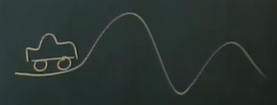
\includegraphics[width=0.4\linewidth]{fig/cruisecontrol}
	\caption{Un automovil necesita tomar en cuenta entradas exógenas como cerros, incertidumbres del modelo y perturbaciones para mantener una velocidad constante.}
	\label{fig:cruisecontrol}
\end{figure}

Un modelo a lazo abierto tiene un controlador de la forma 
\[
\Cu = \MK \Cr
\]
donde $\MK$ es la ganancia del controlador y $\Cr$ es la actuación.

Imaginemos el caso del automovil. Tenemos un sistema SISO (single input, single output), $u$ siendo la potencia erogada por el motor (y los frenos) que es controlada por un actuador. Supongamos que la velocidad es determinada por el input según $y=2u$. Es decir, si queremos una velocidad $y_0$, precisamos la mitad del valor de $y_0$ en actuación para llegar. Si $r$ es el valor de $y$ que se desea llegar, $u_{\openloop}=\frac{1}{2}r$ para un controlador a lazo abierto (LA). 

\begin{figure}[htb!]
	\centering
	\begin{tikzpicture}[auto, node distance=2cm]
		\node[block, label=above:Sistema automovil] (sys) {$y=2u$};
		\node[input,left of=sys,label=below:pot./freno] (in) {};
		\node[block,left of=in] (con) {Controlador};
		\node[input,left of=con,label=below:$y$ deseado] (conin) {};
		\node[output, right of=sys,label=below:velocidad] (out) {};
		\draw[->] (con)-- (in) -- node[above] {$u$} (sys);
		\draw[->] (sys) -- node[above] {$y$} (out);
		\draw[->] (conin) -- node[above] {$r$} (con);
	\end{tikzpicture}
	\caption{Sistema a lazo abierto. Un auto imaginario en buenas condiciones toma una velocidad de dos veces la entrada.}
\end{figure}

Pero puede suceder que se esté intentando controlar un automóvil en condiciones precarias. Si los inyectores no se han limpiado desde hace décadas, tiene ruedas desinfladas, cilindros desgastados, puede suceder que para una entrada $u$ la velocidad sea $y=u$. A lazo abierto nuestro auto anda a mitad de la velocidad de la que se le pide! No es todo, las perturbaciones tendrán un efecto acumulado sobre las incertezas, representadas con $d$. El modelo real del automóvil será diferente al del lazo abierto 

\[
u_\openloop = \frac{r}{2}, \qquad y_{\true} = u + d, \qquad y_\openloop = \frac{r}{2} + d
\]

Como ya habremos visto, los sistemas a lazos cerrados nos dan los beneficios de estabilidad, manejo de incertezas y perturbaciones. La figura \ref{fig:closedloopcruisecontrolexample} implementa un control a lazo cerrado para tal fin.
\begin{figure}[htb!]
	\centering
	\begin{tikzpicture}[auto, node distance=2cm]
	% We start by placing the blocks
	\node [input, name=input] {};
	\node [sum, right of=input] (sum) {};
	\node [blck, right of=sum,label=below:Controlador] (controller) {$K$};
	\node [block, right of=controller,
	node distance=3cm,label=below:Sistema] (system) {$P$};
	\node [sum, right of=system, node distance=2cm,  pin={[pinstyle]above:$d$}] (dist) {};
	\node [output, right of=dist] (output) {};
	
	\draw [->] (controller) -- node[name=u] {$u$} (system);
	\coordinate [below of=u] (tmp);
	\draw [->] (input) -- node {$r$} (sum);
	\draw [->] (sum) -- node {$\error$} (controller);
	\draw [->] (system) -- (dist);
	\draw [->] (dist) --  node [name=y] {$y$}(output);
	\draw [->] (y) |- (tmp) -| node[pos=0.99] {$-$} 
	node [near end] {$y$} (sum);
	\end{tikzpicture}
	\caption{Sistema a lazo cerrado con control proporcional.}
	\label{fig:closedloopcruisecontrolexample}
\end{figure}

En el sistema de la figura aparece el error $\error$ que resulta ser la resta $\error = r-y\closedloop$.

Ahora las ecuaciones que describen el sistema serán
\begin{IEEEeqnarray*}{c}
u_\closedloop = K\error = K(r-y)  \\
y_\closedloop = Pu +d 
\end{IEEEeqnarray*}

Sustituyendo se llega a que $y_\closedloop = PKr - PKy_\closedloop + d$. Resolviendo para $y_\closedloop$
\begin{IEEEeqnarray*}{c}
y_\closedloop = \underbrace{\frac{PK}{1+PK}}_{\text{I}}r + \underbrace{\frac{1}{1+PK}}_{\text{II}}d
\end{IEEEeqnarray*}

El término I nos dice que tan bien la salida $y_\closedloop$ se iguala a $r$ (el valor deseado de $y$). El término II nos dice que tanto las perturbaciones son reducidas por el lazo de control. Recuerde que lo que queremos es que $y_\closedloop=r$, esto se puede lograr aumentando $K$ para que el término I se iguale a 1 y el término II se vaya a cero. Tal vez le resulte escandaloso al lector que con un lazo tan simple el aumento de $K$ indiscriminado mejore el rechazo de perturbaciones y convergencia a $r$, es importante saber que no viene sin sus desventajas.

Desventajas de control proporcional
\begin{itemize}
	\item $K$ esta limitado por el actuador de la realidad. No podemos esperar que el automovil consuma 10 litros de nafta en 1 segundo para llevar $y$ a $r$.
	\item Retardo en la medición puede ocasionar inestabilidad/oscilaciones si $K$ es muy grande. Incertidumbres del sistema también pueden ser nocivas con el aumento de $K$.
	\item En la ausencia de perturbaciones siempre va haber un pequeño error en régimen estacionario. Esto se debe a que el término I llega cerca pero nunca es igual a 1. Ejemplo: Para $PK=100$ va haber un error estacionario del $1\%$. Para remediar esto se puede implementar un integrador
\end{itemize}

\section{Control Integrador}

\begin{figure}[htb!]
	\centering
	\begin{tikzpicture}[auto, node distance=1.5cm]
		\node [block ,label=below:Sistema] (sys) {$P$};
		\node [input, name=sysin, left of=sys] {};
		\node [sum, left of=sysin] (syssum) {+};
		\coordinate[left of=syssum] (gainaux) {};
		\node [blck, above of=gainaux,label=below:Proporcional] (prop) {$K_P$};
		\node [blck, below of=gainaux,label=below:Integrador] (int) {$K_I\, \int$};
		\coordinate [left of=gainaux] (error);
		\node [sum, left of=error, node distance=1cm] (errorsum) {};
		\node [input, left of=errorsum] (rin) {};
		\node [sum, right of=sys,pin={[pinstyle]above:$d$}, node distance=2cm] (dist) {};
		\node[output, right of=dist] (out) {};
		\coordinate [below of=int] (feedback);
		
		\draw [->] (errorsum) -- node {$\error$} (error) |- (prop);
		\draw [->] (prop)  -| (syssum);
		\draw [->] (error) |- (int);
		\draw [->] (int)  -| (syssum);
		\draw [->] (syssum) -- node {$u$} (sys);
		\draw [->] (sys) -- node[pos=.99] {$+$} (dist);
		\draw [->] (dist) -- node[name=y] {$y$} (out);
		\draw [->] (y) |- (feedback) -| node[pos=.99] {$-$} node [near end] {$y$} (errorsum);
		\draw [->] (rin) -- node {$r$} (errorsum);
	\end{tikzpicture}
	\caption{Sistema a lazo cerrado con control proporcional.}
	\label{fig:picontroller}
\end{figure}


La ley de control para el sistema de la figura \ref{fig:picontroller}
\begin{IEEEeqnarray*}{c}
u(t) = K_P(r-y)  + K_I \overbrace{\int_0^t (r-y)\diff \tau}^{=z}
\end{IEEEeqnarray*}

Las integrales en sistemas de control tienen la función de guardar en memoria el los estados anteriores del sistema. Se requiere entonces armar una ecuación auxiliar para cada integral

\begin{IEEEeqnarray*}{c,l}
\dot{x} &= -x -K_Px + K_Iz + K_P r\\
\dot{z} &= r - x \\
u &= K_P (r-x) + K_I z
\end{IEEEeqnarray*}

Las ecuaciones del controlador quedarían en forma matricial
%\todo{Segun un comentario el -1 de la segunda fila primera columna deberia ser positivo...}
\begin{IEEEeqnarray*}{c,l}
\frac{\diff}{\diff t} \begin{bmatrix}
x \\ z
\end{bmatrix} &=
\begin{bmatrix}
-1-K_P& K_I \\
-1 &  0 
\end{bmatrix} 
\begin{bmatrix}
x \\ z
\end{bmatrix}
+
\begin{bmatrix}
K_P \\
1
\end{bmatrix} r \\
y &= \begin{bmatrix}
1 & 0
\end{bmatrix}
\begin{bmatrix}
x \\ z
\end{bmatrix}
\end{IEEEeqnarray*}

Lo que hemos aprendido es que aumentando el espacio de variables con una variable $z$ para el integrador e implementandolo en el lazo de control podemos reducir el error en régimen estacionario a 0 y además converger más rápido a $r$.




\section{Sensibilidad y sensibilidad complementaria}

\begin{figure}[htb!]
	\centering
	\begin{tikzpicture}[auto, node distance=1.5cm]
	\node [block ,label=below:Sistema] (sys) {$\MP$};
	\node [input, name=sysin, left of=sys] {};
	\node [blck, left of=sysin] (con) {$\MK$};
	\coordinate [left of=con] (error);
	
	\node [sum, left of=error, node distance=1cm] (errorsum) {};
	\node [input, left of=errorsum] (rin) {};
	\node [sum, right of=sys, node distance=2.5cm] (dist) {};
	\node [blck, above of=dist,pin={[pinstyle]above:$\Cd$}] (distmat) {$\MP_d$};
	\node[output, right of=dist] (out) {};
	\node [sum,below of=sys,
	pin={[pinstyle]below:$\Cn$}, node distance=2.2cm] (noise) {};
	\node [boxin,label=above:{Lazo $\ML=\MP\MK$}, fit=(sys) (con)] (box) {};
	
	\draw [->] (errorsum) -- node {$\error$} (error) -- (con);
	\draw [->] (con)  -- node {$\Cu$} (sys);
	\draw [->] (sys) -- node[pos=.99] {$+$} (dist);
	\draw [->] (dist) -- node[name=y] {$\Cy$} (out);
	\draw [->] (distmat) -- (dist);
	\draw [->] (y) |- node[pos=.99] {$+$} (noise) -| node[pos=.99] {$-$} node [near end] {$\Cy_m$} (errorsum);
	\draw [->] (rin) -- node {$\Cr$} (errorsum);
	\end{tikzpicture}
	\caption{$\Cy_m$ es el vector de mediciones el cual es afectado por el ruido $\Cn$.}
	\label{fig:loopdaloop}
\end{figure}


La función de transferencia del lazo $\ML=\MP \MK$ va ser el sujeto de estudio. Cuando se trabaja con transferencias es importante el orden de multiplicación. Como indica la figura, la primer función de transferencia en actuar (en el caso del lazo, $\MK$) va estar al final del producto. Ya no estamos hablando de escalares tampoco, estas funciones de transferencia son matrices que operan sobre vectores de error, entrada y perturbaciones.

El objetivo de la realimentación es 

\begin{description}
	\item[Diseñar] estabilidad
	\item[Compensar] incertidumbre del sistema
	\item[Rechazar] perturbaciones
	\item[Attenuar] ruido
\end{description}

El controlador, especificamente, la transferencia $\MK$ estará encargada de que al error $\error$ no le lleguen ruido, perturbaciones.

De la figura \ref{fig:loopdaloop} se obtiene
\begin{IEEEeqnarray*}{c}
\Cy_m=\eye \Cy_m = \MP_d \Cd + \MP \MK \overbrace{(\Cr - \Cy_m - \Cn)}^{=\error} \\
\left(\eye+ \MP\MK\right)\Cy_m = \MP \MK \Cr + \MP_d \Cd \\
\Cy_m = \underbrace{\left(\eye + \MP\MK\right)^{-1} \MP \MK}_{\text{I}} \Cr + \underbrace{\left(\eye + \MP\MK\right)^{-1}}_{\text{II}} \MP_d \Cd- \underbrace{\left(\eye + \MP\MK\right)^{-1} \MP\MK}_{\text{III}} \Cn
\end{IEEEeqnarray*}

Durante el curso de los próximos capítulos se va querer diseñar una ganancia $\MK$ para que: el término I sea cercano a 1 así podemos rastrear la referencia con poco error a bajas frecuencias, el término II sea pequeño para frecuencias donde esperamos perturbaciones, y que el término III sea pequeño para frecuencias donde esperamos obtener ruido (probablemente a altas frecuencias).

El término II se llama la transferencia de sensibilidad \eqref{eq:sensitivity} e indica que tan sensible es el vector salida $\Cy$ a las perturbaciones. El término $\left(\eye + \MP\MK\right)^{-1} \MP \MK$ es la sensibilidad complementaria \eqref{eq:sensitivityCompl} que es asociada a la referencia y al ruido.
\begin{IEEEeqnarray}{c,l}
\ML &= \MP \MK \\
\MS &= \left(\eye + \ML\right)^{-1} \\ \label{eq:sensitivity}
\MT &= \left(\eye + \ML\right)^{-1} \ML\label{eq:sensitivityCompl}
\end{IEEEeqnarray}
una identidad demostrable con álgebra lineal que resulta de estas transferencias es 
\begin{IEEEeqnarray}{c}
\MS + \MT = \eye    \qquad \forall s \in \mathbb{C}
\end{IEEEeqnarray}

Lo más interesante de todo esto es la forma de representar el error a partir de la sensibilidad ya que es lo que se quiere reducir

\begin{IEEEeqnarray}{c}
\error = \Cr - \Cy_m = \MS\Cr - \MS \MP_d \Cd + \MT \Cn
\end{IEEEeqnarray}














%!TeX root = ../control_rapido.tex
%!TeX spellcheck = es_ES
\chapter{Anexo}

\section{Métodos numéricos para resolución de SEDO}

\subsection{Runge--Kutta orden 4 multivariable} \label{sec:metodosNumericos}
El método de Runge Kutta tiene su ventajas sobre otros métodos numéricos por ser simple de programar y tener bajo error ($\error = O(\dt^4)$), donde $\dt$ es el paso elegido. El primer paso consiste en describir el sistema de $\dimss$ variables de forma similar a como hacemos con nuestros sistemas lineales,

\begin{IEEEeqnarray}{c}
\Cx^{\prime} = \Cf (\Cx)
\end{IEEEeqnarray}
que es lo mismo que escribir
\begin{IEEEeqnarray*}{lc}
x_1^{\prime} &= f_1(x_1,x_2,\ldots,x_{\dimss}) \\
x_2^{\prime} &= f_2(x_1,x_2,\ldots,x_{\dimss}) \\
&\vdots \\
x_\dimss^{\prime} &= f_\dimss(x_1,x_2,\ldots,x_{\dimss}) \\
\end{IEEEeqnarray*}

Ahora se definen dos instantes de tiempo $\ts{\Cx}{k}$ de valores conocidos y $\ts{\Cx}{k+1}$ desconocido. Para calcular los valores de $\ts{\Cx}{k+1}$ el algoritmo Runge--Kutta hace lo siguiente

\begin{IEEEeqnarray}{c}
\begin{cases}
\ts{\Ca}{k} &= \Cf(\ts{\Cx}{k}) \\
\ts{\Cb}{k} &= \Cf(\ts{\Cx}{k} + \tfrac{h}{2} \ts{\Ca}{k} ) \\
\ts{\Cc}{k} &= \Cf(\ts{\Cx}{k} + \tfrac{h}{2} \ts{\Cb}{k} ) \\
\ts{\Cd}{k} &= \Cf(\ts{\Cx}{k} + h \ts{\Cc}{k} ) \\
\end{cases} \\
\ts{\Cx}{k+1} = \ts{\Cx}{k} + \frac{h}{6} \left( \ts{\Ca}{k} + 2\ts{\Cb}{k} + 2\ts{\Cc}{k} + \ts{\Cd}{k}\right)
\end{IEEEeqnarray}

El nuevo vector $\ts{\Cx}{k+1}$ te da el estado del sistema después de un pequeño paso $h$.

\bibliography{tex/biblio} % Indica archivo de bibliografia

\end{document}